\documentclass{beamer}
\usetheme{}
\usecolortheme{dolphin}           
\useinnertheme{circles}
\setbeamertemplate{itemize items}[default]
\setbeamertemplate{enumerate items}[default]
\usepackage[T1]{fontenc}
\usepackage[utf8]{inputenc}
\usepackage{lmodern}
\usepackage{amsmath}
\usepackage{booktabs} 
\usepackage{graphicx}        
\usepackage{array}
\usepackage{color}
\makeatletter
\def\zapcolorreset{\let\reset@color\relax\ignorespaces}
\def\colorrows#1{\noalign{\aftergroup\zapcolorreset#1}\ignorespaces}
\makeatother
\graphicspath{{/home/swl/Dropbox/ucd/advanced_macro/figures/}} 
\setbeamertemplate{navigation symbols}{}
\setbeamertemplate{footline}[frame number]

%--------------------------------------
\title{Smets-Wouters model}
\author{School of Economics, University College Dublin}
\date{Spring 2018}
\begin{document}

%--------------------------------------
\begin{frame}
 \titlepage
\end{frame}
%--------------------------------------

%--------------------------------------
\begin{frame}
\textbf{Smets \& Wouters} (2007) "Shocks and Frictions in US Business Cycles : A Bayesian DSGE Approach"
 \scalebox{.7}{
  \begin{quote}
    Using a Bayesian likelihood approach, we estimate a dynamic stochastic general equilibrium model for the US economy using seven macroeconomic time series. The model incorporates many types of real and nominal frictions and seven types of structural shocks. We show that this model is able to compete with Bayesian Vector Autoregression models in out-of-sample prediction. We investigate the relative empirical importance of the various frictions. Finally, using the estimated model, we address a number of key issues in business cycle analysis: What are the sources of business cycle fluctuations? Can the model explain the cross correlation between output and inflation? What are the effects of productivity on hours worked? What are the sources of the “Great Moderation”?
  \end{quote}}
\end{frame}
%--------------------------------------

%--------------------------------------
\begin{frame} 
 Main features
 \begin{itemize}
   \item Sticky nominal price and wage settings
   \item Habit formation in consumption and investment adjustment costs
   \item Variable capital utilization and fixed production costs
 \end{itemize}
\end{frame}
%--------------------------------------

%--------------------------------------
\begin{frame}
 Dynamics in model driven by seven orthogonal structural shocks
 \begin{itemize}
   \item TFP shock
   \item Two shocks affecting intertemporal margin
   \begin{itemize}
     \item risk premium, investment-specific technology shock
   \end{itemize}
   \item Two shocks affecting intratemporal margin
   \begin{itemize}
     \item wage and price mark-up shocks
   \end{itemize}
   \item Two policy shocks
   \begin{itemize}
     \item exogenous spending and monetary policy shocks
   \end{itemize}
 \end{itemize}
\end{frame}
%--------------------------------------

%--------------------------------------
\begin{frame}
  \begin{itemize}
    \item Data: US 1966:1-2004:4
    \item Bayesian estimation methodology
    \begin{enumerate}
      \item Maximise log-posterior; estimate mode posterior distribution
      \item Evaluate marginal likelihood; use Metropolis-Hastings algorithm to get posterior
    \end{enumerate}    
  \end{itemize}
  Note use of deterministic growth rate, driven by labour-augmenting technological process
  \begin{itemize}
    \item Means that data does not have to be detrended
  \end{itemize}
\end{frame}
%--------------------------------------

%--------------------------------------
\begin{frame}
 \textbf{Demand side}  
\begin{align}
  y_t = c_y c_t + i_y i_t + z_y z_t + \epsilon_t^g
\end{align}
$y_t$ is GDP\\
$c_t$ is consumption\\ 
$i_t$ is investment\\
$\epsilon_t^g$ is exogenous spending\\
\medskip
$z_t$ is included in the resource constraint because of the assumption that there are costs associated with having high rates of capital utilisation. 
\end{frame}
%--------------------------------------

%--------------------------------------
\begin{frame}
  Variables with subscript $y$ are steady-state shares
  \begin{align}
    c_y=1-g_y-i_y\\
    i_y=(\gamma-1+\delta)k_y\\
    z_y=R^k_*k_y
  \end{align}  
\end{frame}
%--------------------------------------

%--------------------------------------
\begin{frame}  
Exogenous spending is assumed to develop over time according to
\begin{align}
  \epsilon_t^g = \rho\epsilon_{t-1}^g + \eta_t^g + \rho_{ga}\eta_t^a
\end{align}
Exogenous spending is assumed to have two components
\begin{enumerate}
  \item Government spending
  \item Element related to productivity
\end{enumerate} 
\end{frame}
%--------------------------------------

%--------------------------------------
\begin{frame}
  \textbf{Consumption}  
\begin{align}
  c_t = c_1c_{t-1} + (1-c_1) E_t c_{t+1} + c_2(l_t-E_t l_{t+1}) - c_3(r_t - E_t \pi_{t+1} + \epsilon_t^b)
\end{align}
$c_1, c_2, c_3$ are constant parameters (functions of deeper structural parameters)\\
$r_t$ is the interest rate on a one-period safe bond (quarterly)\\ \medskip

$\epsilon_t^b$ is a risk premium shock determining the willingness of a household to hold the one-period bond
\begin{itemize}
  \item Preference shock that influence short-term consumption-saving decisions
\end{itemize}
\begin{align}
  \epsilon_t^b = \rho_b\epsilon_{t-1} + \eta_t^b
\end{align}
\end{frame}
%--------------------------------------

%--------------------------------------
\begin{frame}
  Two other important things concerning consumption equation
\begin{itemize}
  \item Backward looking consumption term represent habit forming
  \item Equation allows for substitution of consumption with labour input
\end{itemize}

\end{frame}
%--------------------------------------

%--------------------------------------
\begin{frame}
  \textbf{Investment}  
\begin{align}
  i_t = i_ti_{t-1} + (1-i_1)E_ti_{t+1} + i_2q_t + \epsilon_t^i
\end{align}
 Main driver of investment: $q_t$
\begin{align}
  q_t = q_1E_tq_{t+1} + (1-q_1)r_{t+1}^k - (r_t - E_t\pi_{t+1} + \epsilon_t^b)
\end{align}
\end{frame}
%--------------------------------------


%--------------------------------------
\begin{frame}
 \textbf{Supply side}  
\begin{align}
  y_t=\phi_p(\alpha k_t^s + (1-\alpha)l_t + \epsilon_t^a)
\end{align}
$y_t$ is GDP\\
$k^s_t$ is capital in use: determined by lagged level of capital and a capacity utilisation variable
\begin{align}
  k_t^s = k_{t-1} + z_t
\end{align}
$l_t$ is labour input\\
$\epsilon_t^a$ is total factor productivity
\end{frame}
%--------------------------------------

%--------------------------------------
\begin{frame}
 $z_t$ linked to marginal productivity of capital; function of capital to labour ratio and the real wage
\begin{align}
  z_t&=z_1r_t^k; z_1=(1-\psi)/ \psi\\
  r_t^k &= -(k_t-l_t) + w_t
\end{align}
\medskip
Total factor productivity evolves over time according to
\begin{align}
  \epsilon_t^a = \rho \epsilon_{t-1}^a + \eta_t^a
\end{align}
\end{frame}
%--------------------------------------

%--------------------------------------
\begin{frame}
 \textbf{Prices}  
\begin{align}
  \mu_t^p = mpl_t-w_t=\alpha(k_t-l_t) + \epsilon_t^a - w_t
\end{align}
 Equation accounts for 
 \begin{enumerate}
   \item Diminishing marginal productivity of capital 
   \item Productivity shocks effect on costs
   \item Real wage
 \end{enumerate}
\end{frame}
%--------------------------------------

%--------------------------------------
\begin{frame}
  \textbf{Inflation}
\begin{align}
  \pi_t = \pi_1\pi_{t-1} +\pi_2 E_t\pi_{t+1} - \pi_3\mu_t^p + \epsilon_t^p
\end{align}
  \begin{itemize}
   \item Adjusted to account for lagged inflation
   \item Most firms will index their prices based on past inflation levels and can only set an optimal price occasionally
 \end{itemize}
\medskip
$\epsilon_t^p$ is a price mark-up disturbance 
\begin{align}
  \epsilon_t^p = \rho^p \epsilon^p_{t-1} + \eta_t^p - \mu_p\eta_{t-1}^p
\end{align}
\medskip
Shock affects both current and lagged inflation in order to get a temporary price level shock. 
\end{frame}
%--------------------------------------

%--------------------------------------
\begin{frame}
 \textbf{Wages}  
  \begin{align}
  \mu_t^w &= w_t - mrs_t\\
  &= w_t - \left( \sigma_l l_t - \frac{1}{1-\lambda/\gamma} (c_t - \lambda/ c_{t-1}) \right)  
\end{align}
 \medskip
$\mu_t^w$ is the wage mark-up 
\begin{itemize}
  \item Gap between real wage and marginal rate of substitution between working and consuming
  \item Sort of sticky: wages adjust gradually to equate the marginal costs and benefits of working
\end{itemize}
\end{frame}
%--------------------------------------

%--------------------------------------
\begin{frame}
\begin{align}
  w_t &= w_1w_{t-1} \\ \nonumber &+ (1-w_1)E_t(w_{t+1} + \pi_{t+1}) \\ \nonumber
  &- w_2\pi_t + w_3\pi_{t-1} - w_4\mu_t^w + \epsilon_t^w   
\end{align}
\begin{align}
  \epsilon_t^w = \rho^w \epsilon^w_{t-1} + \eta_t^w - \mu_w \eta_{t-1}^w
\end{align} 
\end{frame}
%--------------------------------------

%--------------------------------------
\begin{frame}
  \textbf{Monetary policy}
\begin{align}
  r_t = \rho r_{t-1} + (1-\rho)(r_\pi \pi_t + r_y(y_t - y_t^p)) + \\ \nonumber r_{\Delta y} [(y_t - y_t^p) - (y_{t-1} - y_{t-1}^p)] + \epsilon_t^r 
\end{align}
\begin{align}  \epsilon_t^r = \rho^r \epsilon^r_{t-1} + \eta_t^r \end{align}
\medskip
Central bank sets short-term interest rate according to
\begin{enumerate}
  \item Last period's interest rate
  \item Gradual adjustment towards target interest rate
  \begin{itemize}
    \item Depends on inflation and output gap
  \end{itemize}
  \item Output gap growth rate
\end{enumerate}
\medskip
Potential output defined as the level of output that would prevail if prices and wages were fully flexible
\begin{itemize}
  \item  Model effectively needs to be expanded to add shadow flexible-price economy
\end{itemize}
\end{frame}
%--------------------------------------

%--------------------------------------
\begin{frame}
  Fourteen endogenous variables
  \begin{align*}
    y_t,c_t,i,q_t,k_t^s,k_t,z_t,r_t^k,\mu_t^p,\pi_t,u_t^w,l_t,r_t
  \end{align*}
  \medskip
  Seven exogenous disturbances
  \begin{align*}
    \epsilon_t^a,\epsilon_t^i,\epsilon_t^b,\epsilon_t^g,\epsilon_t^p,\epsilon_t^w,\epsilon_t^r
  \end{align*}  
\end{frame}
%--------------------------------------


%--------------------------------------
\begin{frame}
 \textbf{VAR system}
\begin{align}
  Y_t = \begin{pmatrix}
    dlGDP_t \\ dlCONS_t \\ dlINV_t \\ dlWAG_t \\ lHOURS_t \\ dlP_t \\ FEDFUNDS_t
  \end{pmatrix} =
  \begin{pmatrix}
    \overline{\gamma} \\ \overline{\gamma} \\ \overline{\gamma} \\ \overline{\gamma} \\ \overline{l} \\ \overline{\pi} \\ \overline{r}
  \end{pmatrix} +
  \begin{pmatrix}
    y_t-y_{t-1} \\c_t-c_{t-1} \\ i_t-i_{t-1} \\ w_t-w_{t-1} \\ l_t \\ \pi_t \\ r_t
  \end{pmatrix}  
\end{align}
\medskip
  $l$ and $dl$ stand for 100 times log and log-difference.  
\end{frame}
%--------------------------------------

%--------------------------------------
\begin{frame}
  Additional features compared to RBC or NK model:  
\begin{itemize}
  \item Adjustment costs for investment
  \item Capacity utilisation cost
  \item Habit persistence
  \item Price indexation
  \item Wage indexation
  \item All kinds of autocorrelated shock terms
\end{itemize}
\end{frame}
%--------------------------------------

%--------------------------------------
\begin{frame}
  Fixes included to overcome shortcomings previous model: slow things down
  \begin{itemize}
    \item Give random shocks longer lasting effects
    \item Make development of variables more sluggish
  \end{itemize}
  \medskip
  Velocity major shortcoming of RBC: wage/price indexation addresses NK shortcoming
  \begin{itemize}
    \item Failed to deal with inflation persistence
  \end{itemize}
  \medskip
  Adjustment are largely ad hoc: no clear theoretical grounding.
\end{frame}
%--------------------------------------

%--------------------------------------
\begin{frame}
  \textbf{Priors}\\
  Stochastic processes are harmonised as much as possible
  \begin{itemize}
    \item Rather loose priors are used 
    \item Various distributions: Gamma, Gaussian, Beta
  \end{itemize}
  \medskip
  Five parameters are fixed
  \begin{align}
    \gamma &=0.025\\
    g_y &= 18\%\\
    \lambda_w &= 1.5\\
    \epsilon_p&=\epsilon_w=10
  \end{align}  
\end{frame}
%--------------------------------------


%--------------------------------------
\begin{frame}
  \begin{figure}
     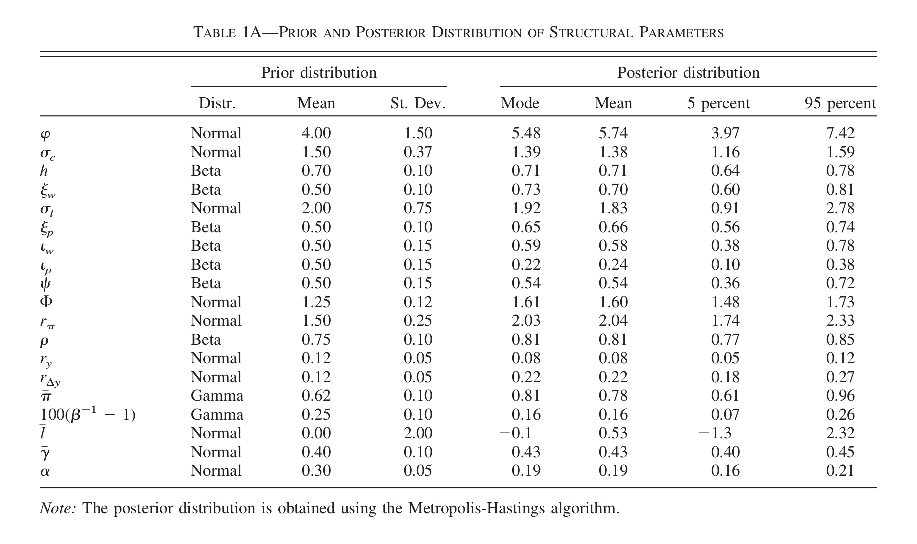
\includegraphics[scale=.7]{sw_table1.eps}
   \end{figure} 
\end{frame}
%--------------------------------------

%--------------------------------------
\begin{frame}
  \begin{figure}
    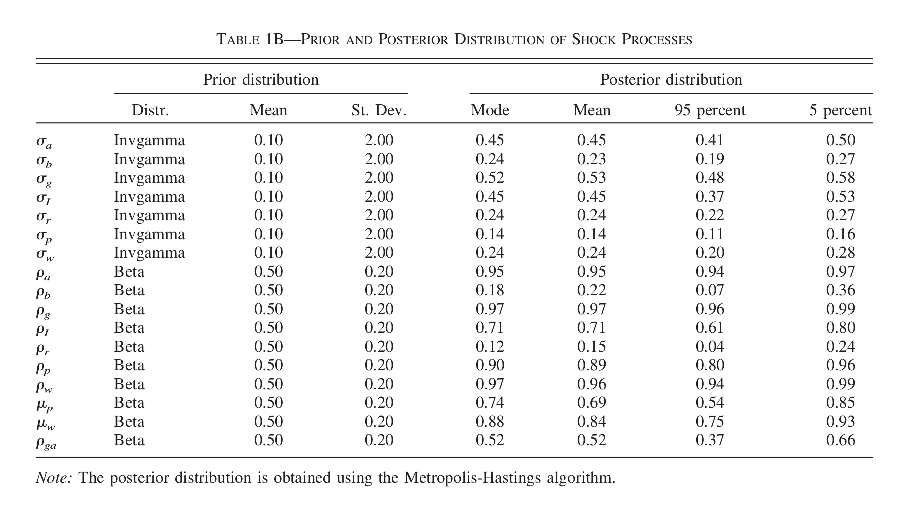
\includegraphics[scale=.7]{sw_table1b.eps}
  \end{figure}
\end{frame}
%--------------------------------------

%--------------------------------------
\begin{frame}
  \textbf{Out-of-sample predictions}
  \begin{enumerate}
    \item Estimate model, using data 1966:1-1989:4
    \item Forecast data series for 1990:1-2004:4
  \end{enumerate}
  \medskip
  VAR models were re-estimated each quarter, DSGE model each year.
\end{frame}
%--------------------------------------

%--------------------------------------
\begin{frame}
  \begin{figure}
    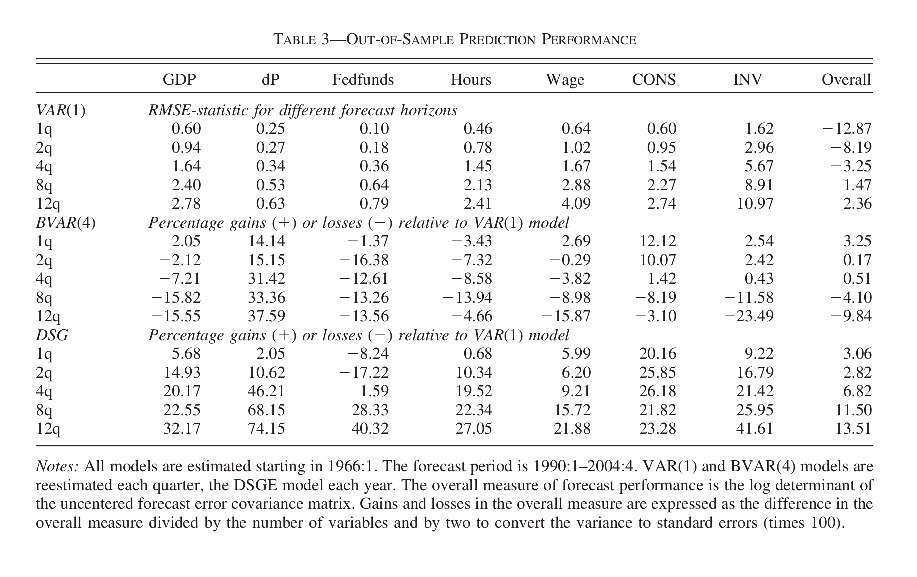
\includegraphics[scale=.7]{sw_table3.eps}
  \end{figure}
\end{frame}
%--------------------------------------

%--------------------------------------
\begin{frame}
  Model is used to answer four questions
  \begin{enumerate}
    \item What are the sources of business cycle fluctuations? 
    \item Can the model explain the cross correlation between output and inflation? 
    \item What are the effects of productivity on hours worked? 
    \item What are the sources of the “Great Moderation”?
  \end{enumerate}
\end{frame}


%--------------------------------------
\begin{frame}
  \begin{figure}
    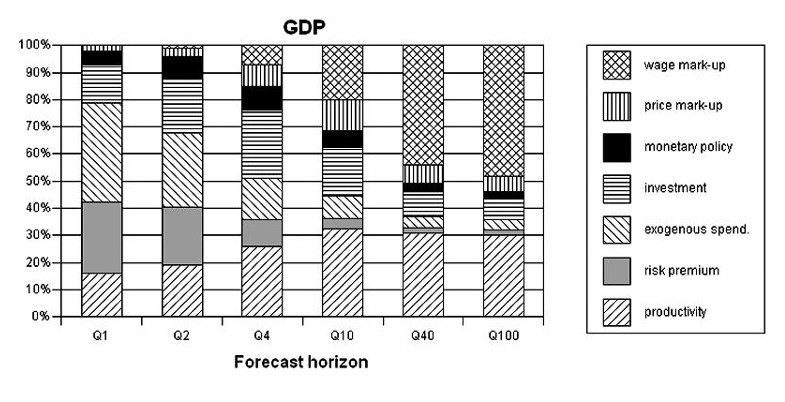
\includegraphics[scale=.8]{sw_figure1_gdp.eps}
  \end{figure}
\end{frame}
%--------------------------------------

%--------------------------------------
\begin{frame}
  \begin{figure}
    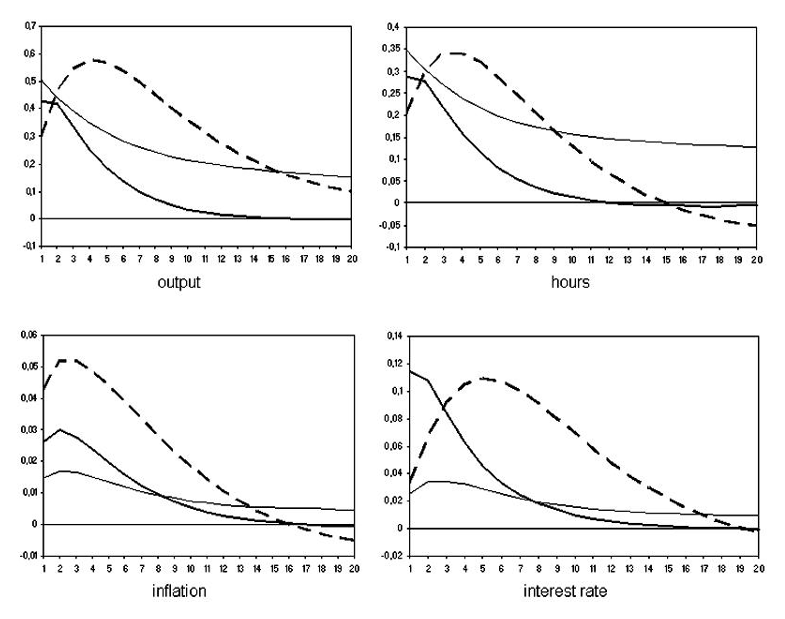
\includegraphics[scale=.8]{sw_figure2.eps}
  \end{figure}
\end{frame}
%--------------------------------------

%--------------------------------------
\begin{frame}
  \begin{figure}
    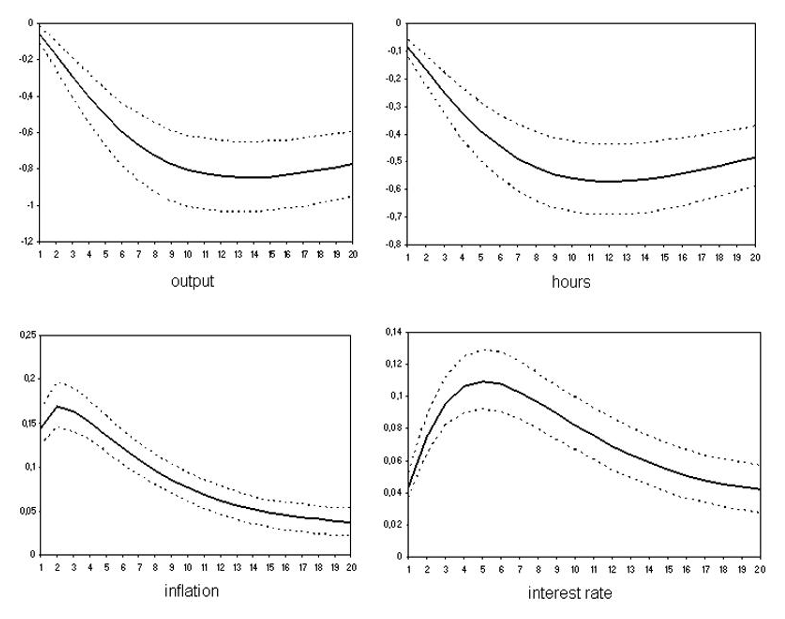
\includegraphics[scale=.8]{sw_figure3.eps}
  \end{figure}
\end{frame}
%--------------------------------------

%--------------------------------------
\begin{frame}
  \begin{figure}
    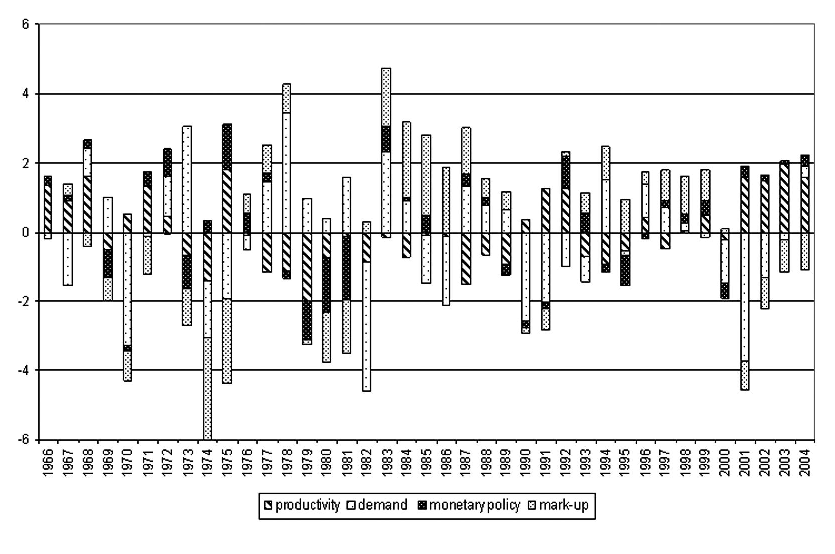
\includegraphics[scale=.8]{sw_figure4_gdp.eps}
  \end{figure}
\end{frame}
%--------------------------------------

%--------------------------------------
\begin{frame}
  \begin{figure}
    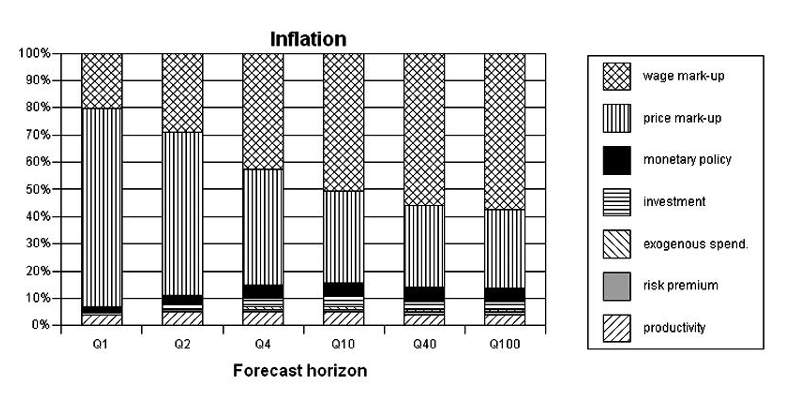
\includegraphics[scale=.8]{sw_figure1_inflation.eps}
  \end{figure}
\end{frame}
%--------------------------------------

%--------------------------------------
\begin{frame}
  \begin{figure}
    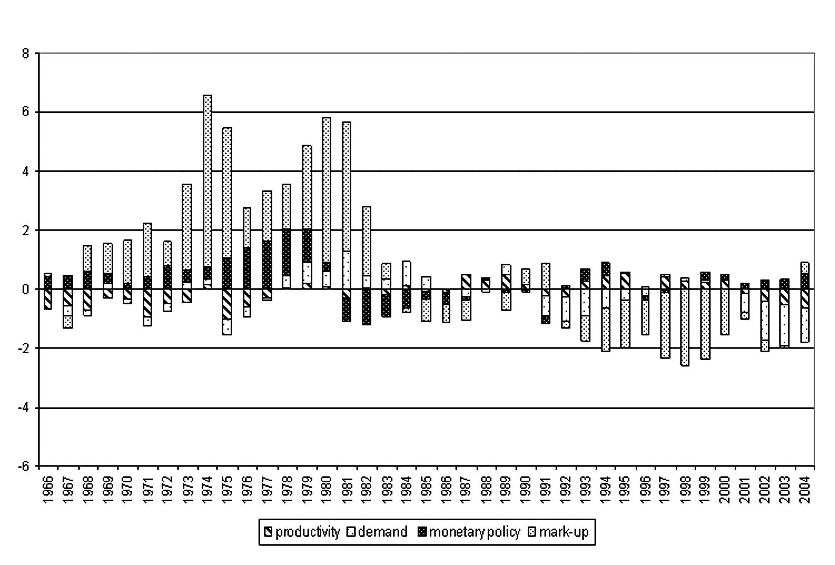
\includegraphics[scale=.8]{sw_figure4_inflation.eps}
  \end{figure}
\end{frame}
%--------------------------------------

%--------------------------------------
\begin{frame}
  Two reasons for limited effect of demand/productivity shocks on inflation
  \begin{enumerate}
    \item Estimated slope NKPC is small
    \item Fed responds aggressively to emerging output gaps and impact on inflation (according to estimation)
  \end{enumerate}
\end{frame}
%--------------------------------------

%--------------------------------------
\begin{frame}
  \begin{figure}
    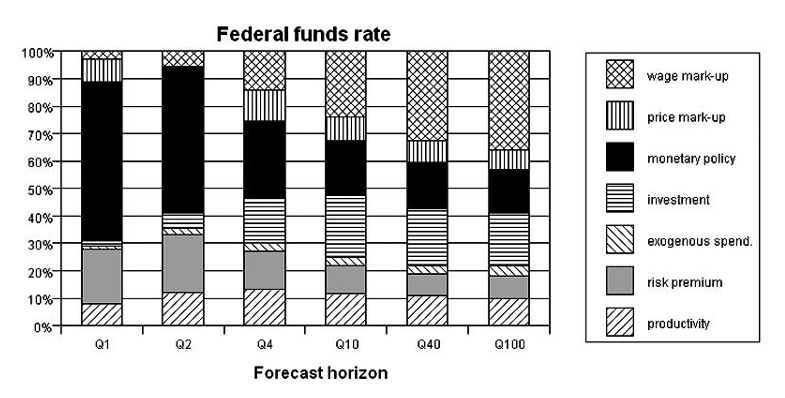
\includegraphics[scale=.8]{sw_figure1_interest.eps}
  \end{figure}
\end{frame}
%--------------------------------------

%--------------------------------------
\begin{frame}
  \begin{figure}
    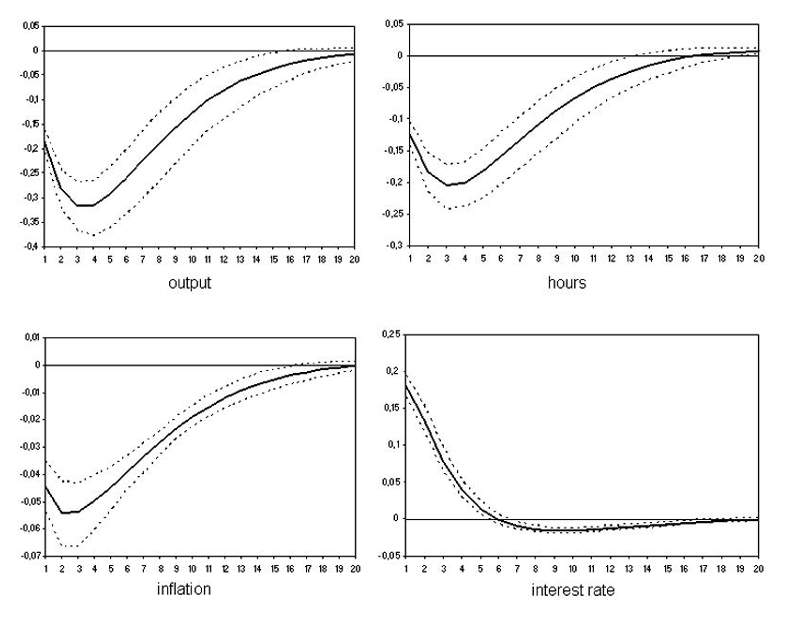
\includegraphics[scale=.8]{sw_figure6.eps}
  \end{figure}
\end{frame}
%--------------------------------------

%--------------------------------------
\begin{frame}
  \begin{figure}
    \includegraphics[scale=.4]{sw_figure7.eps}
  \end{figure}
\end{frame}
%--------------------------------------

%--------------------------------------
\begin{frame}
  Test stability of results estimate model for two subsamples
  \begin{enumerate}
    \item Great Inflation 1966:2-1979:2 
    \item Great Moderation 1984:1-2004:4 
  \end{enumerate}
\end{frame}
%--------------------------------------

%--------------------------------------
\begin{frame}
  \begin{figure}
    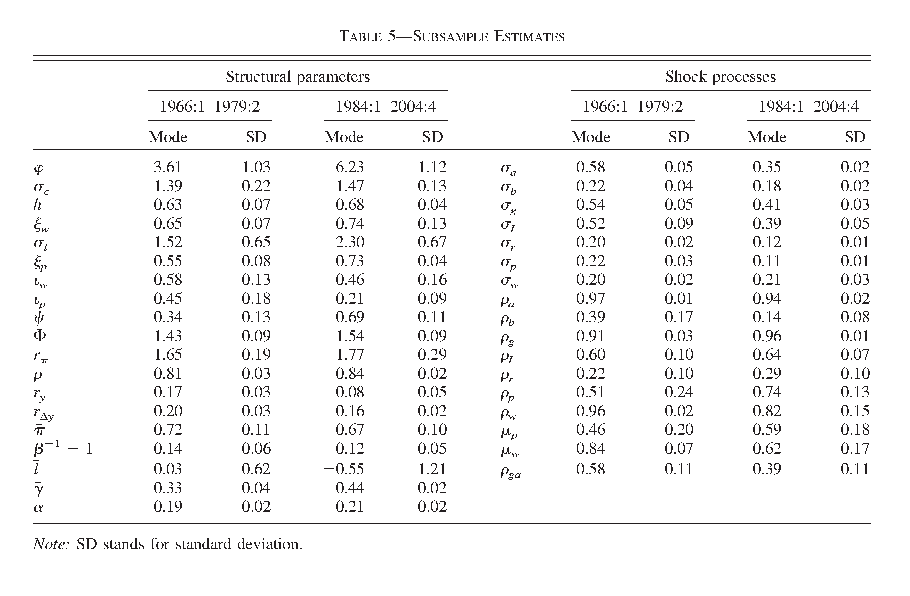
\includegraphics[scale=.7]{sw_table5.eps}
  \end{figure}
\end{frame}
%--------------------------------------

%--------------------------------------
\begin{frame}
  \begin{figure}
    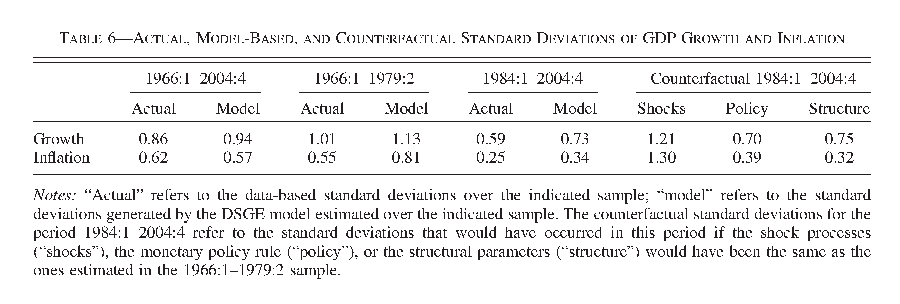
\includegraphics[scale=.7]{sw_table6.eps}
  \end{figure}
\end{frame}
%--------------------------------------

%--------------------------------------
\end{document}
